\chapter{Research Design and Methods} \label{ch:[chapter 5 label]}

\section{Overview}

In this research proposal, I have discussed the problem of search abandonment. I have noted that abandonment is partially due to search systems providing irrelevant results. This is because these systems have a weak understanding and employment of relevance. Guided by my research question, I propose a five-study research design to address this problem and improve our understanding of relevance in GIR. The relationships between studies are illustrated in figure \ref{fig:Methods_Overview}. Specifically, these studies will

\begin{enumerate}
    \item survey existing portals and record the state of faceted  search,
    \item analyze a portal for user search behavior, query topics, and latent concepts in queries that may suggest what users find relevant,
    \item analyze if and how latent concepts change with location (i.e., the location of a portal and/or datasets from a portal),
    \item modify an existing portal's search system to incorporate my findings on concept usage from the previous two studies, and
    \item evaluate the effectiveness of these modifications.
\end{enumerate}

\begin{figure}[H]
    \centering
    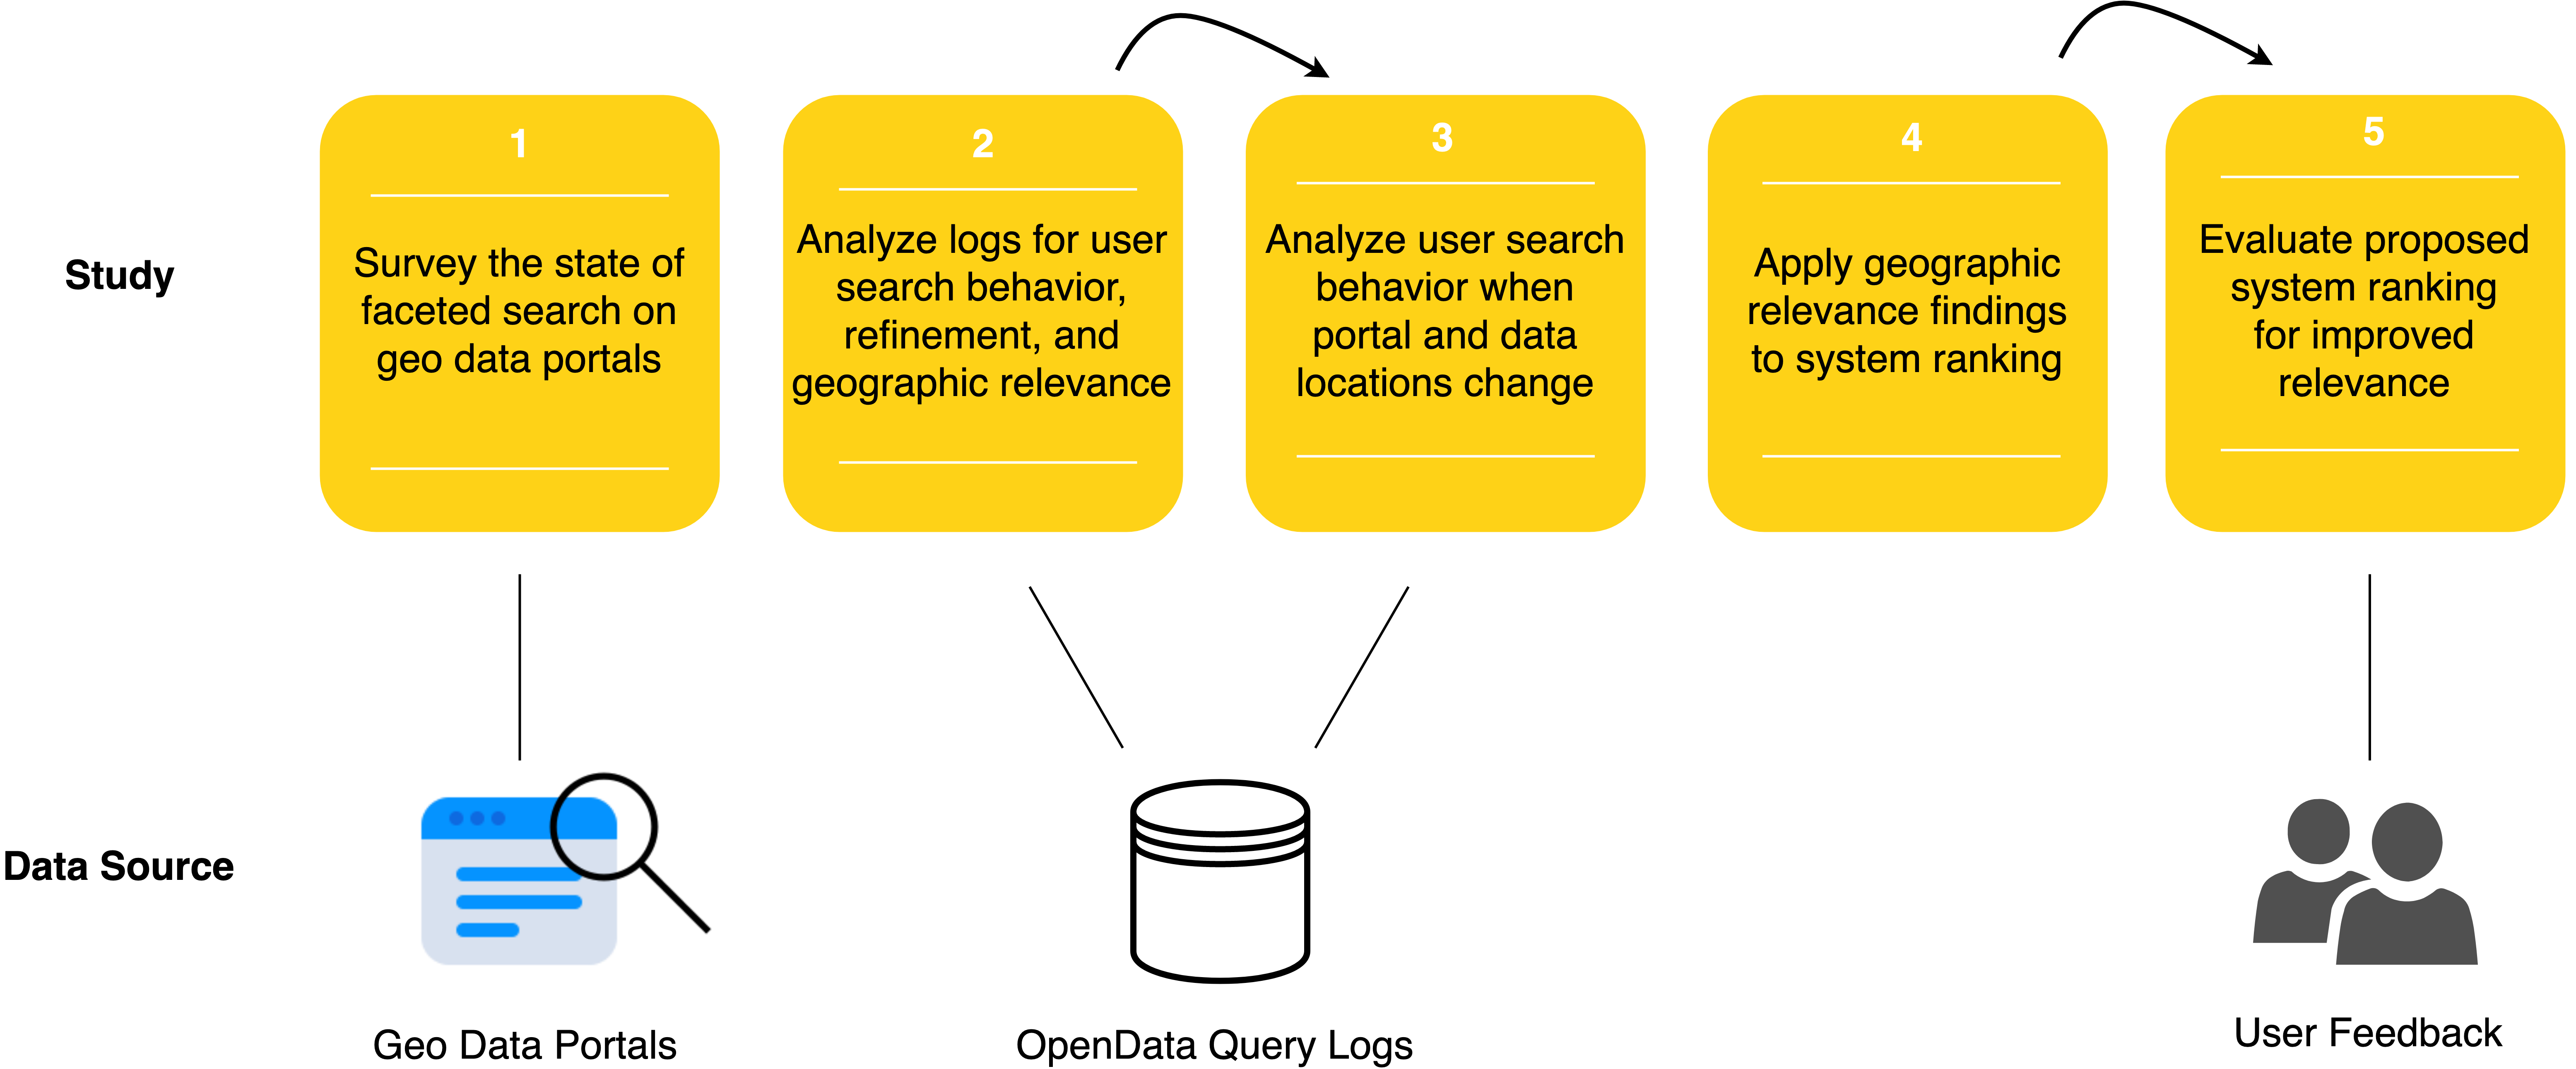
\includegraphics[width=1\textwidth]{../figures/Methods_Overview.png}
    \caption{Overview of research studies and their data sources. Studies progress by purpose including surveying the state of the art, interpreting search behavior, interpreting search behavior when location changes, applying knowledge about behavior, and evaluating the application. Arrows indicate a direct follow-up study.}
    \label{fig:Methods_Overview}
\end{figure}

\section{Surveying the State of Search in Geospatial Data Portals}

\subsection{Study Question}

The first step to reducing search abandonment to establish a baseline for search effectiveness. I am interested in understanding what facets users can control when they search and how search systems interpret and reason on user queries. By learning what portal users can do, I can identify gaps in their search systems. Therefore, my first research question is:
\linebreak

\emph{What is the state of faceted search and scoring/ranking functions on geospatial data portals?}

\subsection{Methods}

To answer this question, I will first survey the search facets of several commercial and academic portals including but not limited to Esri's OpenData, data.gov, census.gov, UCSB's Alexandria Digital Library, UCSB Library's new data portal, and Geoblacklight\footnote{\url{https://geoblacklight.org/}} enabled portals. I will record facets such as filtering by tags, drawing a region of interest on a map, or sorting alphabetically. Figure \ref{fig:Methods_OpenData} highlights the facets that a user controlled when searching and the ordered list of results.

Most search systems on portals do not publish their scoring/ranking functions, but many rely on open source data portals like CKAN\footnote{\url{https://ckan.org/}} and search tools like Apache Lucene\footnote{\url{https://lucene.apache.org/}}. They often leverage simple ranking models built on \gls{tf_idf} (\acrshort{TF_IDF}). TF–IDF ranks a document highly when it has a large number of similar words to a user's query, but those words aren't common in other documents. I expect that these search systems will apply similar functions possibly with minor customizations. For each portal, I will attempt several different information seeking tasks as if I were a typical user. I will simulate searching for data using specific queries for specific tasks. For example, in one scenario, I will simulate that I am a citizen who wants to reappraise their house and needs to find GIS data on parcels (to understand my property boundaries and coverage). After executing a query like "parcels", I will record the top 10 results and iteratively adjust the query to see if results change. Query adjustments will include: addition and removal of non-geographic, geographic, thematic and temporal terms, rearranging of terms, and the introduction and removal of terms indicative of the concepts that I hypothesized as being important. For example, I will add and remove spatial granularity keywords like "county" and "state", and density expressions such as "dense" or "even". Since data sparsity is likely to be an issue on some portals, I will trace several specific datasets on each portal and see how query adjustments affect their ranking.

\subsection{Expected Outcome}
The expected outcomes of this study will be threefold. First, this study will produce a list of observed options that affects search results on portals. This list will include all search facets and search weights, when knowable. A highly usable system strikes a balance between user control and system control. Systems with a large number of user controls dissuade serendipity, but few controls give little guidance. Second, this study will produce qualitative descriptions of how altering search terms affects results. Comparing queries and their responses will show if and how systems handle keywords differently. Third, this study will describe the observed deficiencies in existing systems including what queries and search facets yields irrelevant results, if any.

\begin{figure}[H]
    \centering
    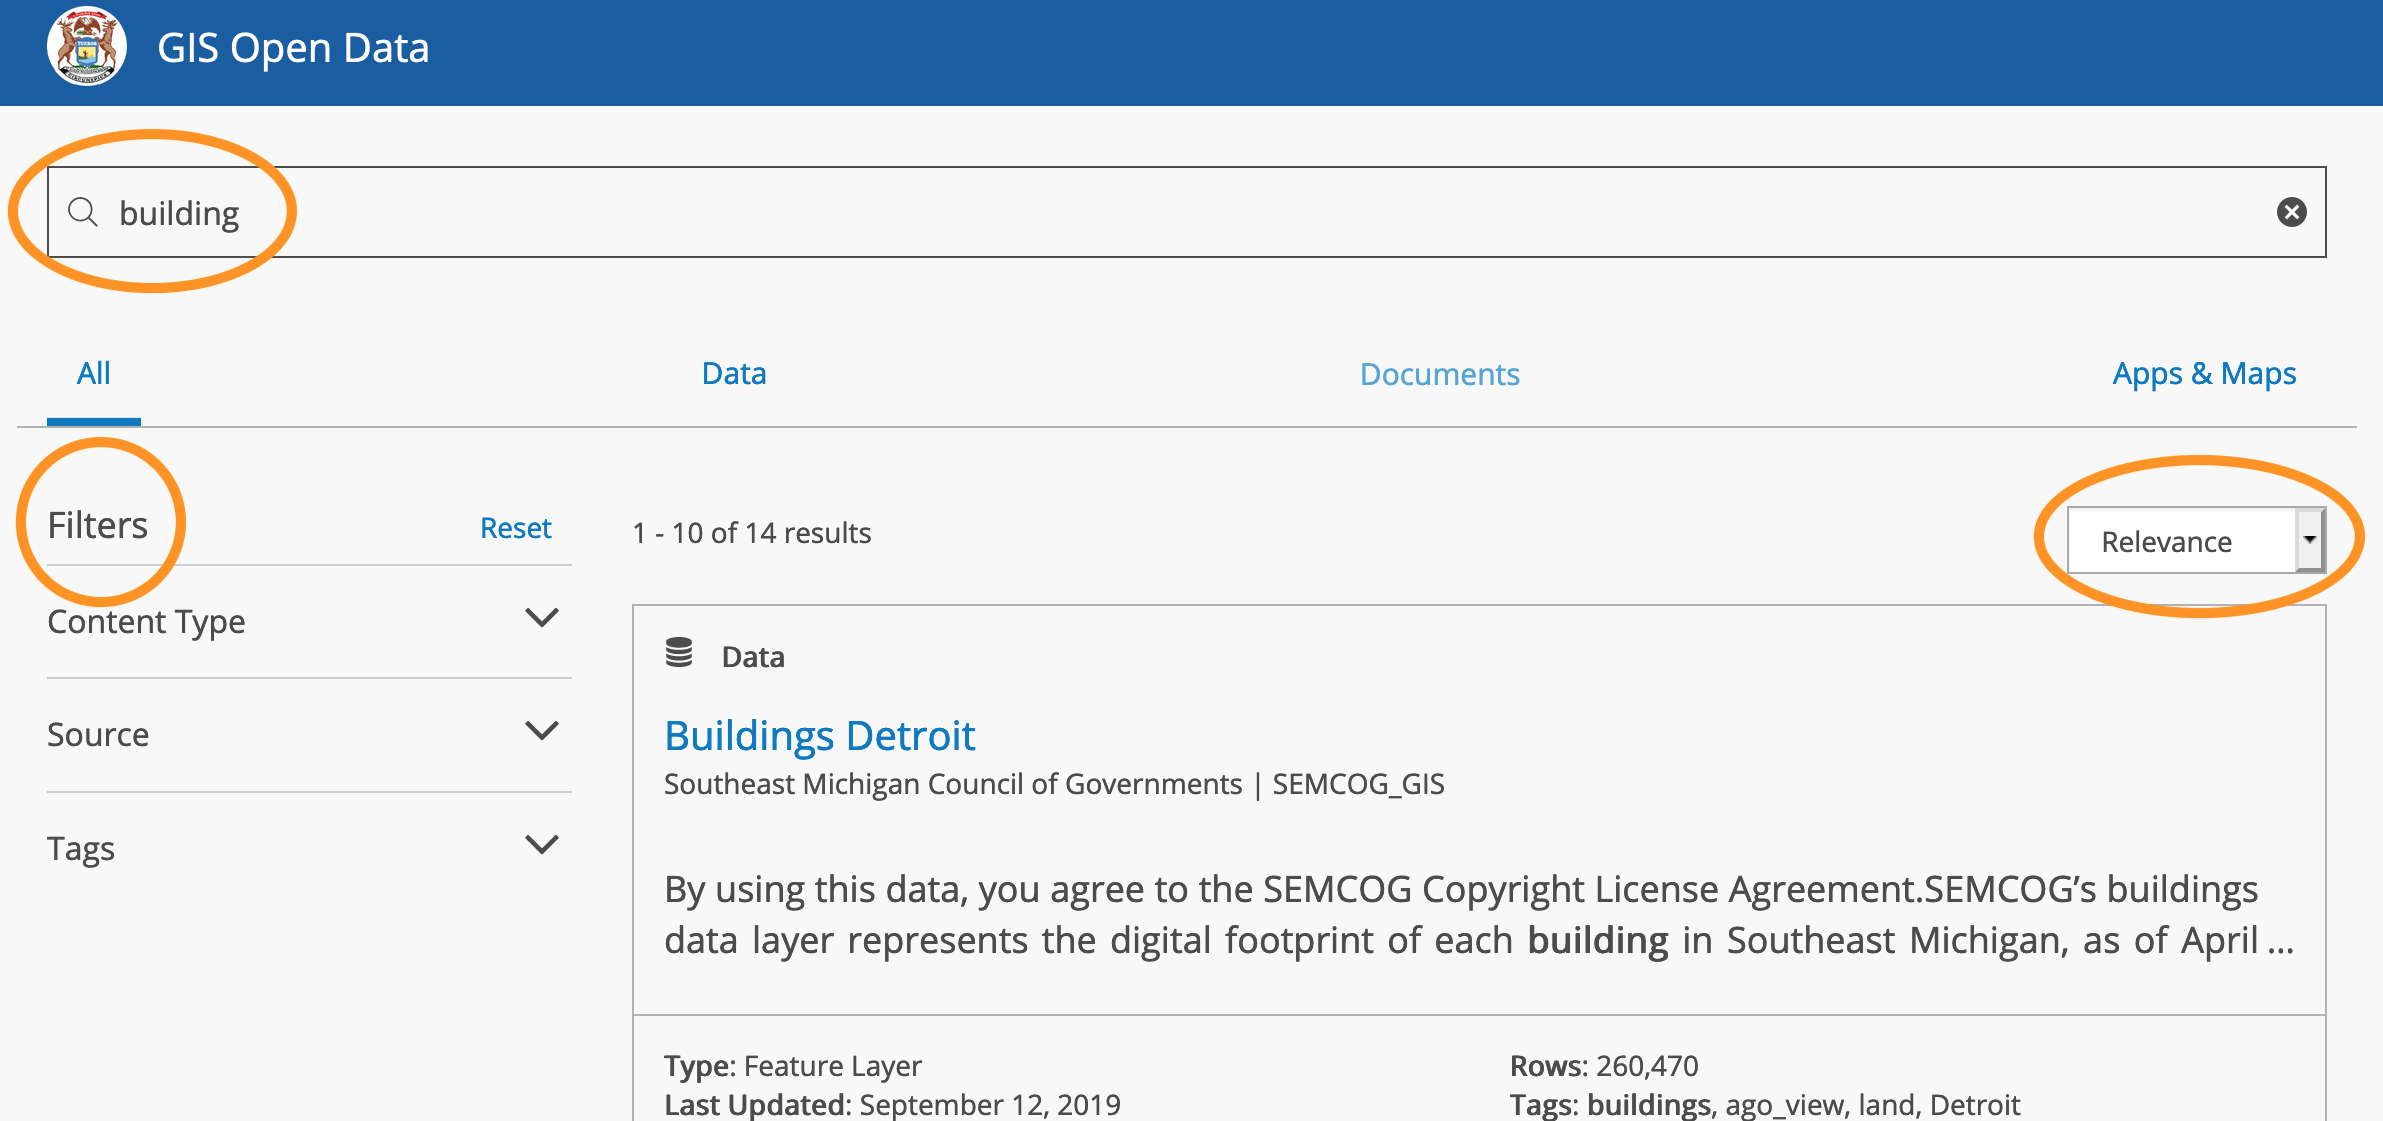
\includegraphics[width=1\textwidth]{../figures/Methods_OpenData.png}
    \caption{An example SERP from the Michigan OpenData portal. Orange highlights indicate facets that users control when searching. Surveying facets, surveying scoring/ranking functions, and observing SERP result changes from query changes are the research objectives of study 1. An ordered list of results are seen bottom right.}
    \label{fig:Methods_OpenData}
\end{figure}

\section{Search Behavior, Refinement and User's Query Concepts on Esri’s Geospatial OpenData Portals}
\subsection{Study Question}
\subsection{Data}
\subsection{Methods}
\subsection{Expected Outcome}

\section{Impacts of Location on Search Behavior in Search of Geographic  Datasets}
\subsection{Study Question}
\subsection{Data}
\subsection{Methods}
\subsection{Expected Outcome}

\section{An Experimental Study on the Effectiveness of Introducing Relevance Criteria in Geographic Information Retrieval}
\subsection{Study Question}
\subsection{Data}
\subsection{Methods}
\subsection{Expected Outcome}

\section{Evaluating the Effectiveness of a Geographically-Oriented Search Rank Algorithm}
\subsection{Study Question}
\subsection{Data}
\subsection{Methods}

Figure \ref{fig:Methods_Evaluation}

\subsection{Expected Outcome}

\begin{figure}[H]
    \centering
    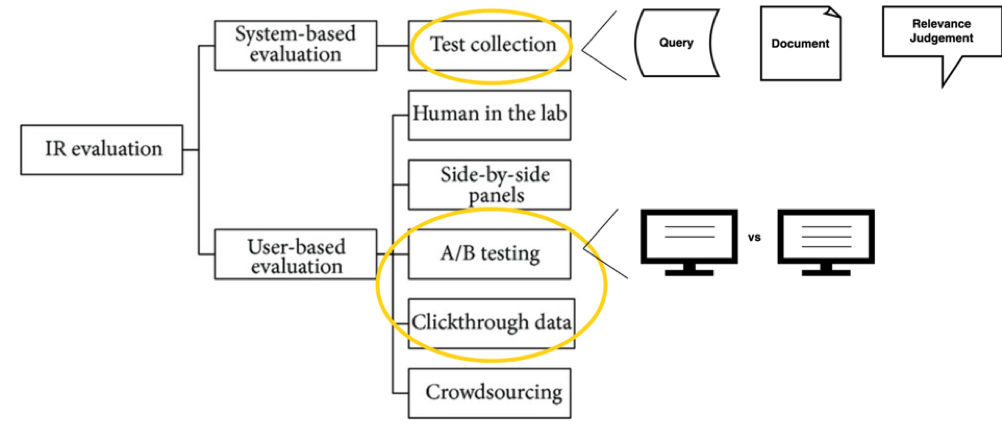
\includegraphics[width=1\textwidth]{../figures/Methods_Evaluation.png}
    \caption{Classification of IR evaluation approaches adapted from \cite{Samimi2014}. Yellow highlights indicate the evaluation approaches used in this study. A test collection comprises a query, document, and relevance judgement for each query-document pair. A/B testing assigns users to either an A (control) or B (modified) search system and compares their behavior. I will also add an option for self-reported relevance on each SERP result. Click-through data, parsed from query logs in study 2, will be used to cross-reference A/B testing results.}
    \label{fig:Methods_Evaluation}
\end{figure}